\documentclass[a4paper,12pt]{article}
\usepackage[utf8]{inputenc}
\usepackage{amssymb,amsmath,uniinput,graphicx,hyperref, multirow,siunitx}
\usepackage[section]{placeins}
\usepackage[ngerman]{babel}
\usepackage[left=3cm,right=3cm,top=3cm,bottom=3cm]{geometry}
\renewcommand{\familydefault}{\sfdefault}
\setlength{\belowcaptionskip}{6pt}
\hypersetup{pdfinfo = {
	Title={Versuchsprotokoll zu Positronen im Festkörper},
	Author={Knut Kiesel, Tobias Pook},
	Keywords={Positronen Teufel Ananas}
}}


\graphicspath{{../pictures/}{../analyse/}}
\title{Laborpraktikum Teilchenphysik\\ Lebensdauer von Positronen im Festkörper}
\author{Knut Kiesel\\Tobias Pook}
\date{\today}

\begin{document}
\maketitle
\vspace{3cm}
\tableofcontents
\thispagestyle{empty}
\newpage
\setcounter{page}{1}

\section{Ziel des Versuches}
Ziel des Versuches ist der Aufbau und die Inbetriebnahme einer Messstation,
die in der Lage ist die Lebensdauer von Positronen in Festkörpern in der
Größenordnung von $\SI{100}{ps}$ zu messen.

Da die Annihilationswahrscheinlichkeit von der Energie abhängig ist,
müssen die Positronen thermalisiert werden.
Dies dauert bei Aluminium wenige $\si{ps}$.
In Isolatoren oder amorphen Stoffen dauert die Abbremszeit sehr viel länger,
sodass sich das Positron mit einem Elektron des Festkörpers zu einem Positronium verbinden können,
wenn die Affinitäten von Elektron und Positron kleiner
als die Affinität von Positronium und dessen Bindungsenergie ist.
Hier gibt es zwei Möglichkeiten: Parapositronium mit entgegengesetztem Spin und Orthopositronium mit gleichgerichtetem Spin.
Orthopositronium hat eine längere Lebensdauer, weil es nur in drei Photonen zerfallen kann, was unwahrscheinlicher als der Zerfall in zwei Photonen ist.
Durch Elektronenaustausch wandelt es sich oft in Parapositronium um, welches durch den Zerfall in zwei Photonen eine kürzere Lebenszeit hat.

Als Positronenquelle wird in diesem Versuch $^{22}$Na verwendet, welches beim Zerfall in $^{22}$Ne
zuerst ein γ-Quant der Energie $\SI{1.28}{MeV}$ abgibt und dann ein Positron emittiert.
Nach einer vom Festkörper abhängigen Zeit annihiliert das Positron unter Aussendung
von zwei bis drei γ-Quanten mit einer Energie von $\SI{511}{keV}$.
Durch das messen der Zeitdifferenz zwischen dem ersten γ-Quant des Übergangs und dem
γ aus der Annihilation kann die Lebensdauer des Positrons bestimmt werden.


\section{Aufbau und Durchführung}
%Kommentare aus der Vorbesprechung:
%	Constant Fraction Discriminator liefert logisches out bei BLD Ausgang
%	Die Delay Einheit ändert die polarität des Signal, wenn gewünscht.
%	Der Multi Channel Analyzer nimmt nur positive Signal ohne Offset an.

Der Detektor, zu sehen in Abbildung \ref{fig:quelle},  besteht aus zwei zylindrischen Szintiallatonsdetektoren,
welche in einem Gehäuse mit einem Photomultiplier verbaut sind.
\begin{figure}[htb]
		\centering
		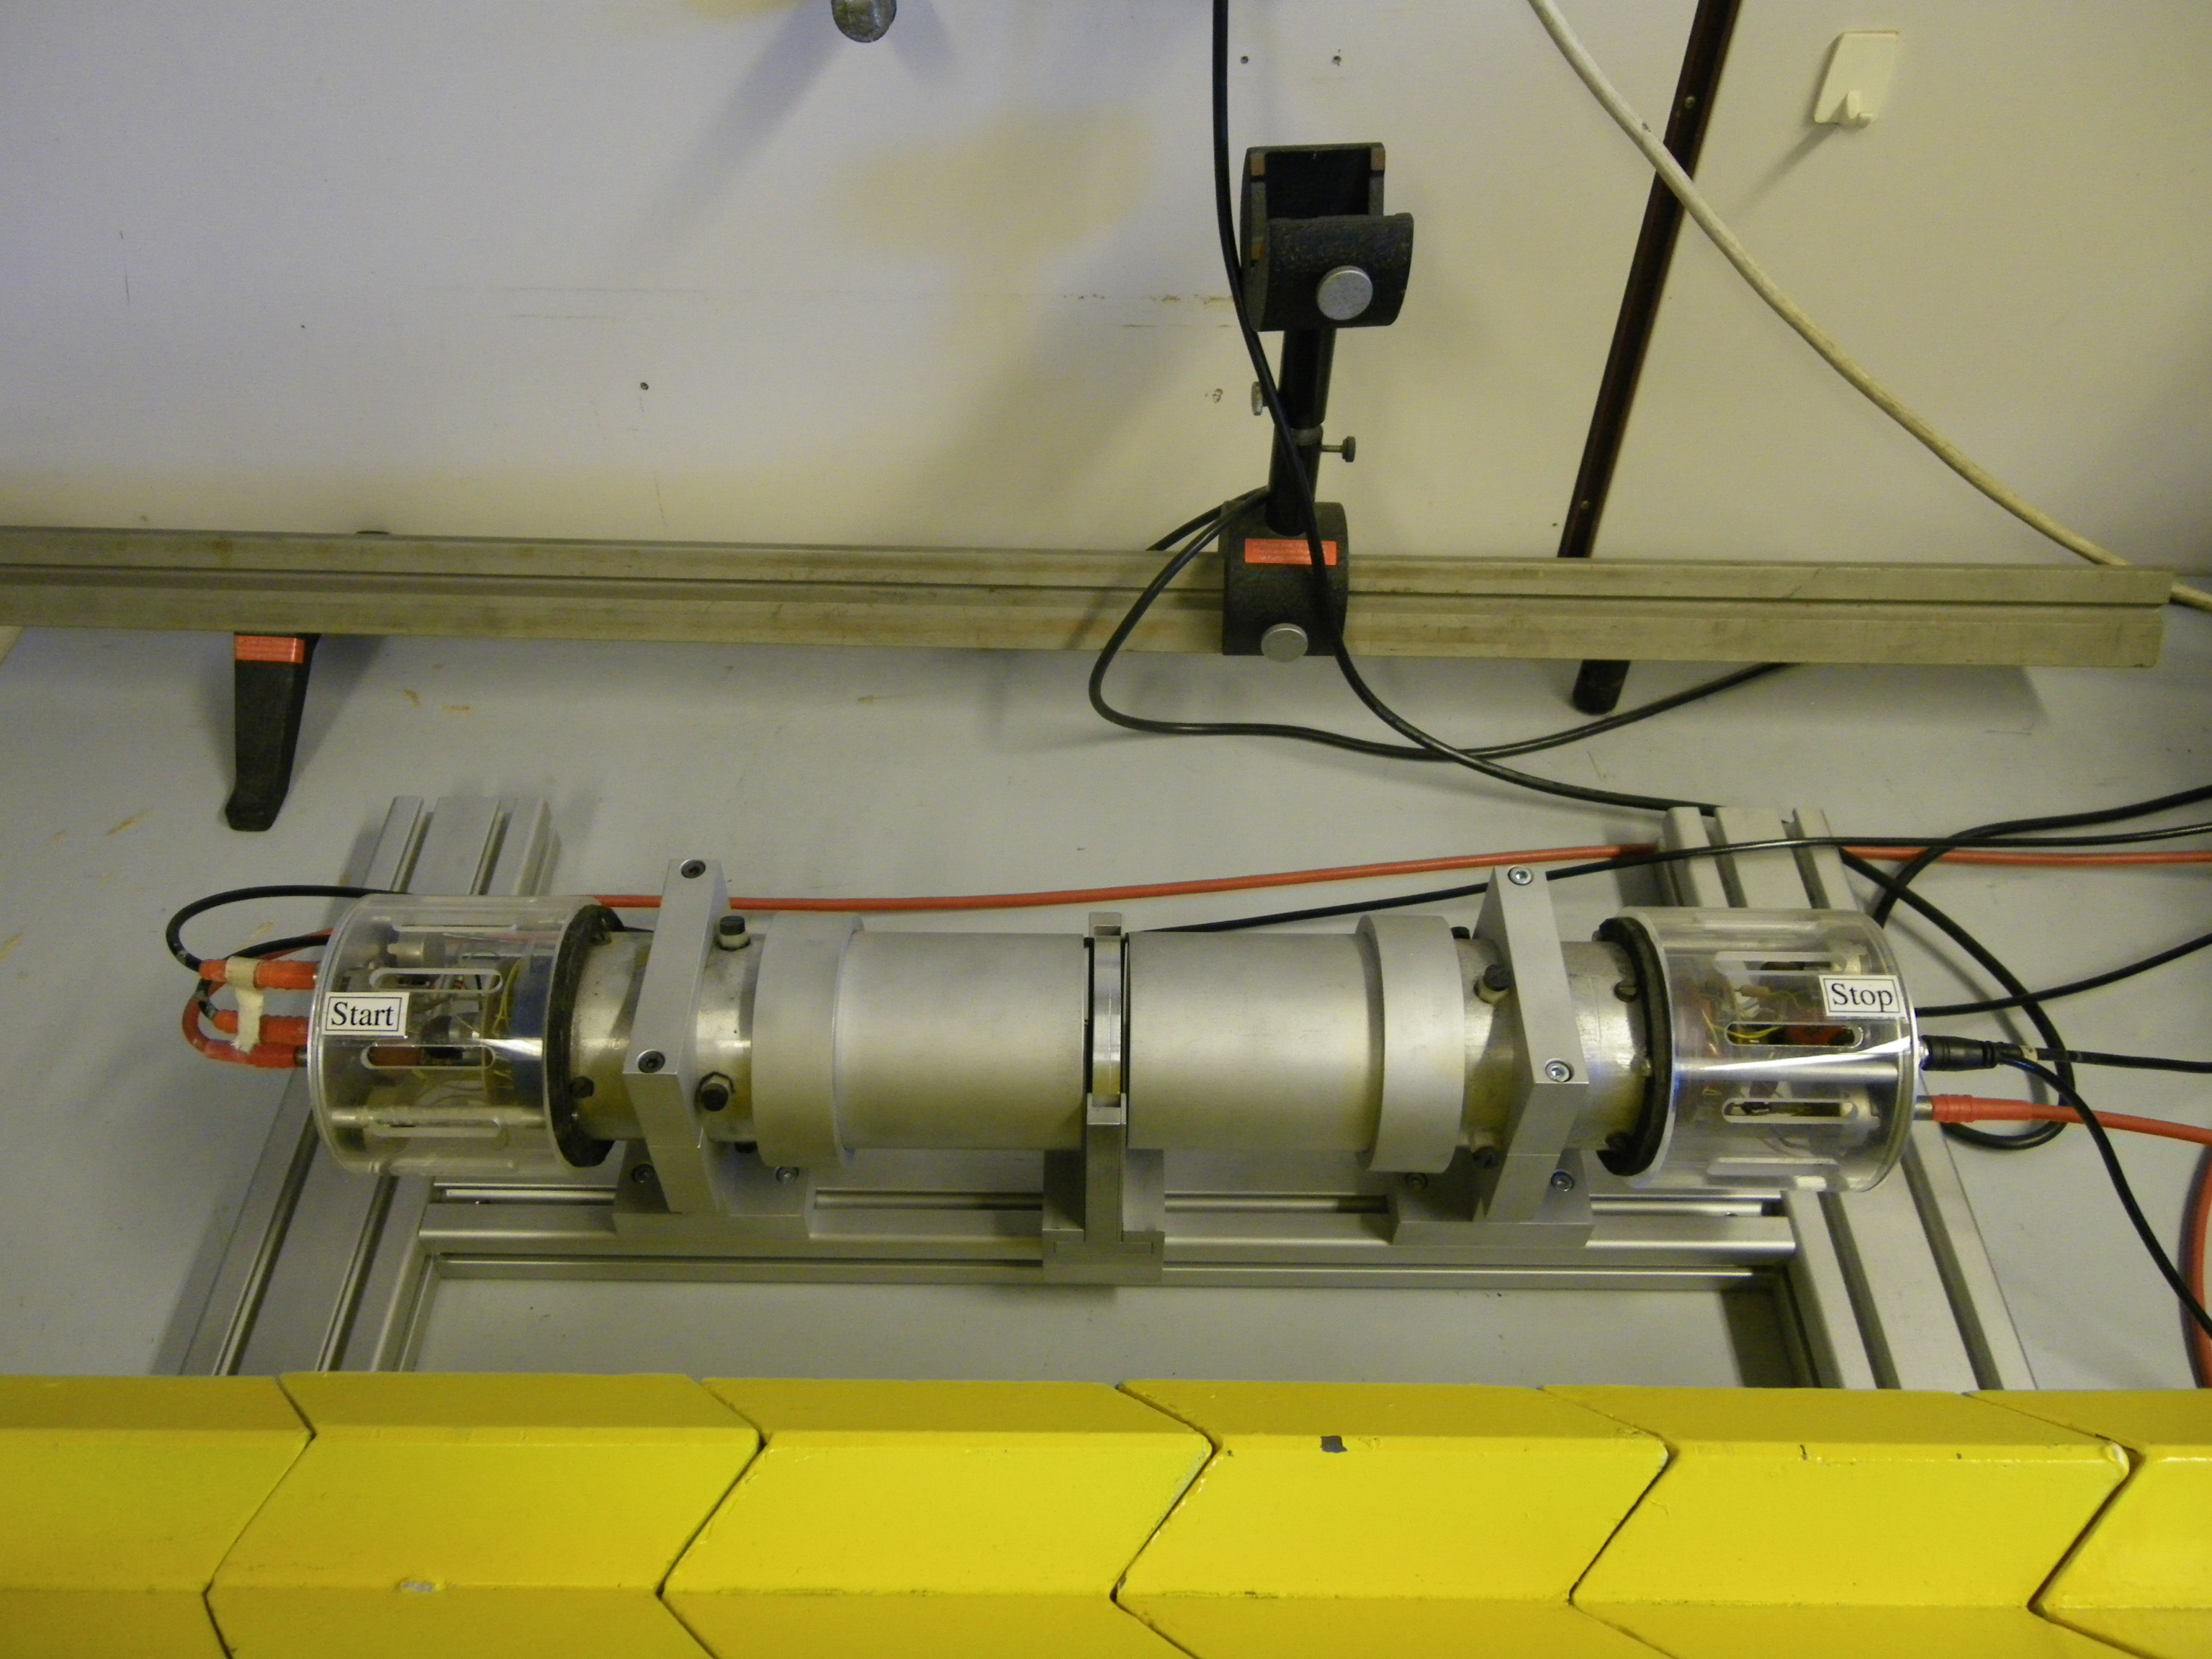
\includegraphics[width=0.5\textwidth]{quelle2.jpg}
		\caption{Scintilatoren mit Photomultiplier und Quelle}
		\label{fig:quelle}
\end{figure}

Die radioaktiven Proben werden zwischen beiden Szintillatoren platziert.
An der Katode des Photomultipliers wird  eine Spannung von von $\SI{-2}{kV}$ angelegt.
Damit sind die Anodensignale noch nicht übersättigt.
Von beiden Photomultipliern wird sowohl das Anodensignal als auch das Dynodensignal, also das Signal an der letzten Dynode, abgegriffen.
Das Dynodensignal ist ein leicht positives Signal, dessen Pulse aus stark schwankenden kleineren Pulsen besteht, trotzdem aber eine Höhe hat, die Energie abhängig ist.
Das Signal wird für die Energiemessung und damit für das Gate verwendet.

Das Anodensignal ist ein Puls mit negativem Ausschlag und eine der Energie entsprechenden Höhe.
Es wird für das Messen der Zeitabstände benutzt, da das Dynodensignal mit den starken Schwankungen genaue schnelle Messungen von kleinen Zeitabständen nicht zulässt.

Es liefert für das Dynoden- und das Anodensignal jeweils ein Photomultiplier das Start und der andere das Stoppsignal.

Durch die Trennung in Anodensignal und Dynodensignal kann man den Schaltkreis in zwei unabhängige Kreise unterteilen, die nur an einer Stelle wieder zusammenlaufen.
Sie werden "`schneller"' und "`langsamer"' Kreis genannt.

Der Aufbau beider Schaltkreise ist in Abbildung \ref{fig:aufbau} zu sehen.
\begin{figure}[htb]
		\centering
		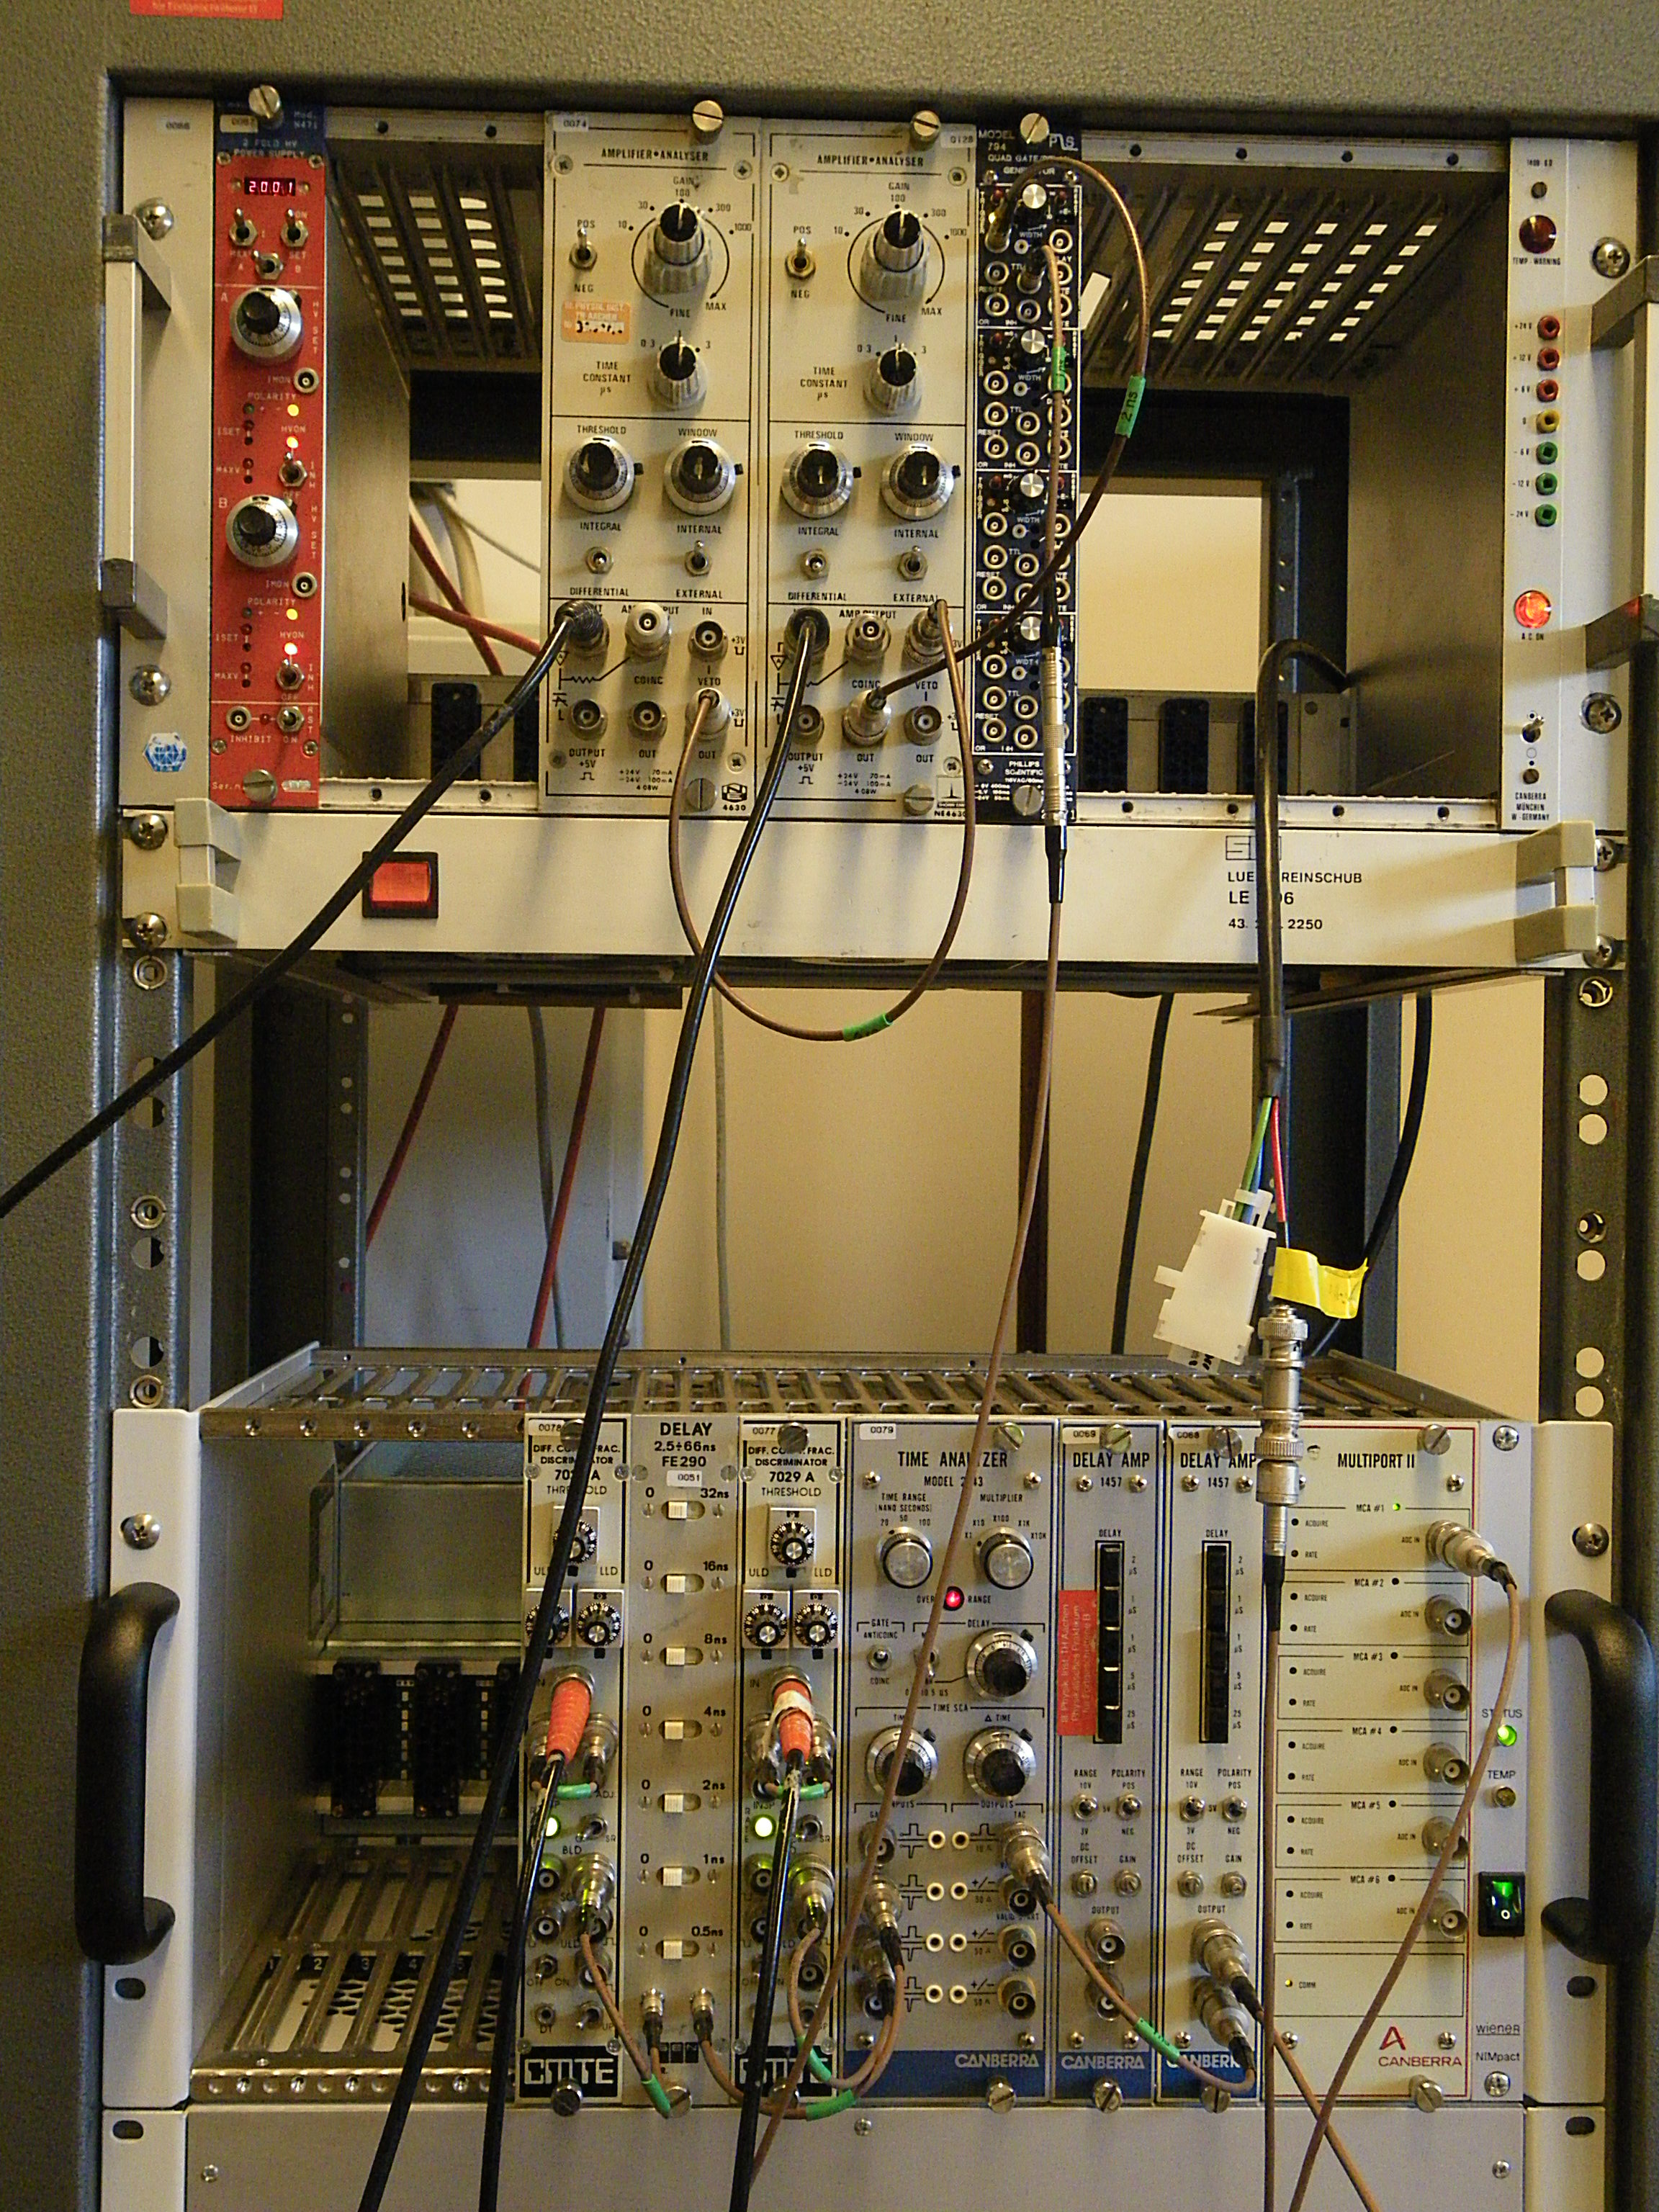
\includegraphics[width=.5\textwidth]{aufbau.jpg}
		\caption{Photo der elektronischen Verschaltung}
		\label{fig:aufbau}
\end{figure}

Links oben befindet sich die rote Spannungsquelle, daneben zwei Amplifier Analyzer mit Koinzidenzstufe\footnote{Nuclear Enterprises, Modell 4630} für Start und Stopsignal des langsamen Kreises.
Als letztes in der oberen Reihe ist das ein Quad Gate\footnote{Fa. Phillips Scientific, Modell 794} zu sehen.

In der unteren Reihe umgeben zwei Differential Constant Fraction Discriminatoren\footnote{Fa. Stanford Research Systems Inc., Modell DG535} eine Delay Einheit\footnote{Fa. SEN, Modell FE290}.
Rechts daneben befindet sich ein Time Analyser\footnote{Fa. Canberra, Modell 2043}, zwei Delaystufen\footnote{DFa. Canberra, Modell 1457} und zuletzt ein Vielkanalanalysator\footnote{Multiport II, Fa. Canberra} der auf der Rückseite mit einem Computer und dem Gate verbunden ist.

Schematisch ist der Aufbau in Abbildung \ref{fig:schaltplan} zu sehen.
\begin{figure}[htb]
		\centering
		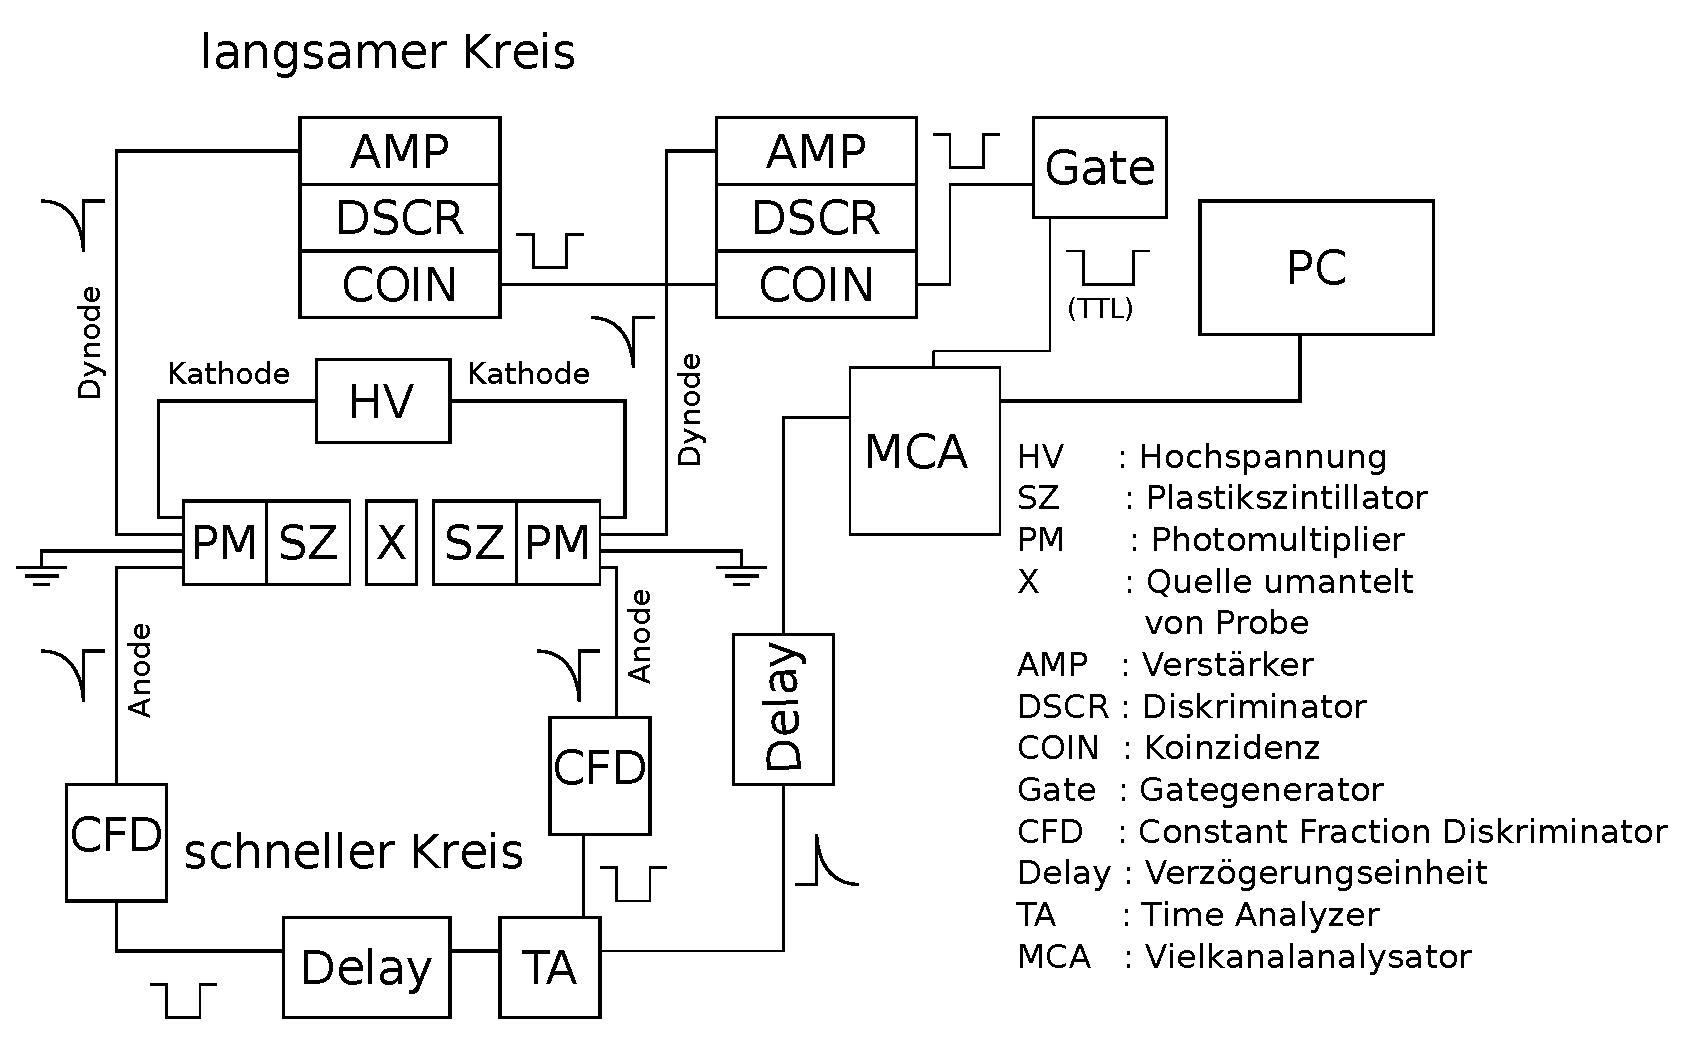
\includegraphics[width=1.0\textwidth]{Schaltplan_custom.pdf}
		\caption{Schematischer Schaltplan des Aufbaus des Versuchs.
		An den Seiten sind die Signalformen (logisch/analog) angegeben.}
		\label{fig:schaltplan}
\end{figure}

Wie schon oben genannt und wie auch in der Abbildung zu sehen, wird der Schaltkreis in zwei Kreise unterteilt:
\begin{itemize}
	\item
	Der langsame Kreis prüft ob sich die gemessenen Photonen sich im richtigen Energieintervall 
	befinden und erzeugt abhängig davon ein Triggersignal, das das Gate des Vielkanalanalysators öffnet.
	\item
		Der schnelle Kreis bestimmt die Zeitdifferenz und gibt dieses in Form eines Pulses an den
	Vielkananlanalysator weiter.
\end{itemize}
\subsection*{Langsamer Kreis}
Für den langsamen Kreis wird das Dynodensignal der Photomultiplier genutzt und in jeweils einem
Einzelkanaldiskriminator (\textbf{EKD}) weiter verarbeitet.
Dieser verstärkt das Signal zunächst (es wird ein Gain von 300 eingestellt),
damit sich das Energiespektrum im Vielkanalanalysator über möglichst alle Kanäle erstreckt.
% Erklären was beim Differenzieren passiert.
Das Dynodensignal besitzt eine ausreichende Abhängigkeit zwischen Energie und Pulshöhe
um ein (nicht kalibriertes) Energiespektrum mit Hilfe des Vielkanalanalysator aufzuzeichnen.

Anschließend werden die Schwellwerte des Diskriminators im EKD so eingestellt,
dass nur Teilchen mit einer höheren Energie als die rechten Flanke des Anhilationspeak als
Startsignal (Fenster 2 in Abbildung \ref{fig:auswahl}) genutzt werden
und Teilchen in einem niedrigeren Energiefenster als Stoppsignal.

Wenn ein Teilchen im richtigen Energiefester ist, wird an einem Ausgang ein logisches Signal erzeugt,
was über das Gate zusammen mit dem verstärkten Dynodensignal in den Vielkanalanalysator geleitet wird.

Um eine Ober-und Untergrenze zu setzen, muss das Signal zuvor Differenziert werden,
was auch mit diesem Gerät möglich ist\cite{linearAmplifier}.

Das Stopsignal soll bei einer Annihilation eines Positrons entstehen
und deshalb eine Energie von $\SI{511}{keV}$ haben.
In Abbildung \ref{fig:auswahl} ist dies Fenster 1.
Zusätzlich wird eine untere Grenze bei 260±10
eingestellt um den Untergrund durch niederenergetischer Teilchen und elektronisches Rauschen des Photomultipliers zu reduzieren.
Die obere Grenze bei Kanal 3640±30 ist gleichzeitig die Grenze für das Startsignal,
bei dem ein $\SI{1.28}{MeV}$ Photon erwartet wird.
Diese Grenze ist sehr viel ungenauer,
da das Setzen des Schwellenwerts nicht für einen steilen Abbruch des Spektrums sorgt, sondern nur für ein weiches Abfallen.
% Time constant = 1μs
% threshold1 = 20 window = 340
% threshold = 350, window = 1000 (max)
% differential mode


% erkläre veto-out und veto-in, was genau machen die, und warum fuktioniert das?
Nachdem die Fenster für Start und Stoppsignal zunächst mit dem verstärkten Dynodensignal eingestellt sind,
wird der logische 'Veto-Out' Ausgang des Start-EKD in den 'Veto-In' Eingang des Stop-EKD gesteckt und das logische Ausgangssignal über das Gate
in den Vielkanalanalysator gegeben.
Die EKD dienen damit auch gleichzeitig als Koinsidenzstufen.

\begin{figure}[h]
	\centering
	\includegraphics[width=0.8\textwidth]{../analyse/auswahl.pdf}
	\caption{Das Energiespektrum von $^{22}$Na aus dem verstärktem und vorgeglätteten
		Dynodensignal.
		Man sieht von rechts nach links bei Kanal 10000 den Peak des $\SI{1.28}{MeV}$ Photons,
		danach das Comptonkontinuum und bei etwa Kanal 3500 den Annihilationspeak.
		Am linken Rand (Kanal kleiner als 260) sieht man Rauschen, das ignoriert wird.
		Für ein Startsignal (Fenster 2) muss das ein größerer Kanal als 3630±100 angesprochen werden, 
		für ein Stopsignal ( Fenster 1) reicht ein Kanal größer als 260±10.}
	\label{fig:auswahl}
\end{figure}


\subsection*{Schneller Kreis}
Für den schnellen Kreis wird das Anodensigal der Photomultiplier genutzt.
Start und Stoppsignal werden zunächst in jeweils einem Constant
Fraction Discriminator (\textbf{CFD}) weiter verarbeitet.
Dieser erzeugt durch differenzieren zunächst einen bipolaren Puls aus dessen Nulldurchgang ein von der Pulsform unabhängiges Zeitsignal erzeugt wird
und in Form eines logischen Signal ausgegeben wird, wenn eine gewisse Pulshöhenschwelle überschritten wurde.
Um hier die Schwellen zu setzen, wird das logische Signal jeweils eines CFD über das Gate an den Vielkanalanalysator gesendet.
Die eigentliche Energieinformation bekommt man aus der Anode.
Ein Startsignal wird genauso definiert wie beim langsamen Kreis, das Stopsignal wird nur durch eine untere Schranke festgelegt (also Fenster 1 und 2 in Abbildung \ref{fig:auswahl}).
Als Schwellen werden am Gerät schließlich 0.9 bzw 9.0 eingestellt und das Gerät im CF Mode betrieben

Nachdem die Schwellen gesetzt werden, kann das Startsignal in den Starteingang des Timeanalysers, das Stopsignal über ein schnelles Delay, das im Messzustand auf 0 gestellt ist, in den Stopeingang des Timeanalysers.
Der Time Analyzer erzeugt einen Puls, dessen Pulshöhe vom zeitlichen Abstand von Start und Stoppsignal ist.

Im Vielkanalanalysator werden die Pulse in ein Pulshöhenspektrum umgesetzt.
Um den schnellen und langsamen Kreis zeitlich aufeinander 
anzupassen ist zusätzlich eine Verzögerungseinheit zwischen Time Analyzer und den Vielkanalanalyser geschaltet, dessen Zeit auf $\SI{3}{μs}$ gestellt wird.
% time analyser einstellungen:
% gate: anticoincidenz, delay var: 1.9, time: 0.9, delta_T = 10.0

\section{Kalibration des Aufbaus}
Damit mit dem Aufbau Zeitdifferenzen gemessen werden können, muss der Vielkanalanalysator kalibriert
sowie die Zeitauflösung bestimmt werden.
\subsection{Zeitkalibration des Vielkanalanalysators}
Um die einzelnen Kanäle des VKA mit den entsprechenden Zeitabständen zu verknüpfen wird eine Zeitkalibration durchgeführt. Dazu werden
mit einem Pulsgenerator Pulse mit einer Amplitude von $\SI{3}{V}$ und einer Pulsbreite von 10ns mit
einer Frequenz von $\SI{1600}{Hz}$ mit einem 
Plusgenerator\footnote{Four Channel Digital Delay/Pulse Generator, Fa. Stanford research Systems Inc. Modell DG535}
erzeugt.
Es wurde mit einem Oszilloskop sichergestellt, dass Form und Amplitude des erzeugten Puls denen aus dem Anodenausgang der Photomultiplier
entsprechen. Das vom Pulsgenerator ausgegebene Signal wird durch ein T-Stück geteilt. Eine Abzweigung des T-Stück wird in den für das Startsignal vorgesehene
CFD geleitet, die andere in den CFD für das Stoppsignal. Vor der eigentlichen Kalibrierung wird das Delay getestet, indem
das Signal vor und nach dem Delay nicht durch die Constant Fraction Diskriminatoren sondern durch ein Oszilloskop abgegriffen werden. Hier lässt sich erkennen,
dass beide Signale bei ausschalten des Delay nahezu zeitgleich ankommen und in ihrer Pulsform erhalten bleiben. Es kann also ausgeschlossen werden das es zu
zusätzlichen Verzögerungen oder sonstige Verfälschungen des Signal durch das T-Stück und die genutzten Kabel kommt.
Nach dem Testen des Delay wird die ursprüngliche Verschaltung wieder hergestellt und die zeitlichen Abstände der logischen Signale der CFDs im Time Analyzer
in Pulshöhen umgesetzt. Die Pulse des Time Analyzer werden an den Vielkanalanalysator weiter geleitet, dieser wird während der Kalibrierung mit
durchgehend geöffnetem Gate betrieben. Die Verzögerung wird am Delay in $\SI{0.5}{ns}$ Schritten von $\SI{0}{ns}$ bis $\SI{12}{ns}$ erhöht, das aufgezeichnete Pulshöhenspektrum
ist in Abbildung \ref{fig:pulsSpektrum} dargestellt.

\begin{figure}[h]
	\includegraphics[width=\textwidth]{../analyse/peaksToArray.pdf}
	\caption{Pulshöhenspektrum zur Zeitkalibration. Die Pulse haben einen Abstand von
		$\SI{0.5}{ns}$. Man sieht schon hier, dass die Peaks vor allem im unteren Bereich nicht
	äquidistant sind. Die Höhe der Peaks ist nur eine Folge der Dauer, die man mit einer Einstellung
gemessen hat und geht nicht in die Kalibration ein.}
	\label{fig:pulsSpektrum}
\end{figure}


Es wird an jeden Peak  im Spektrum eine Gaußfunktion angepasst.
Für die Anpassung wird die Erwartungswert $μ$ als Mittelwert und die elektronische Zeitauflösung $σ$
als Fehler auf den Mittelwert genommen.
Ein Beispiel für eine solche Anpassung, für einen Zeitabstand von $\SI{8}{ns}$, ist in Abbildung \ref{fig:singlePuls} dargestellt.

\begin{figure}[h]
	\includegraphics[width=\textwidth]{../analyse/singlePeak.pdf}
	\caption{Ein einzelner Puls aus Abbildung \ref{pulsSpektrum} zur genaueren Untersuchung. Der zu
	$\SI{8}{ns}$ gehörende Peak wird durch eine Gaußfunktion gut beschrieben. Die Breite ist typisch
	für die Peaks und liegt zwischen $5$ und $\SI{10}{ns}$.}
	\label{fig:singlePuls}
\end{figure}

Da es keine Möglichkeit (wie zum Beispiel den Vergleich mit einem weiteren Delay) gab, die Unsicherheit auf die genutzten Verzögerungen zu bestimmen und es auch keine Angaben zu
 den Unsicherheiten in der Betriebsanweisung des Bauteil zu finden waren wurde der Fehler auf die
 Verzögerung zu 15\% der Schrittweite von $\SI{0.5}{ns}$ abgeschätzt.
 An die so gewonnenen Zeit-Kanal Wertepaare wird in Abbildung \ref{fig:kalibrationsRegression} mittels linearer Regression eine Gerade angepasst, mit der im folgenden
Kanalnummern in Zeitabstände umgerechnet werden.

\begin{figure}
	\includegraphics[width=\textwidth]{linearRegression.pdf}
	\caption{Lineare Regression zur Zeitkalibration des Vielkanalanalysators. Die Fehler auf die
	Kanalnummern sind vernachlässigbar, da die elektronische Auflösung sehr gut ist. Die Fehler auf
die Zeiten der Delayeinheit überwiegen immer.}
	\label{fig:kalibrationsRegression}
\end{figure}

Da die Daten für kleine Kanalnummern nicht durch eine Gerade beschrieben werden können, wird die
Anpassung erst ab Kanalnummer $4000$ vorgenommen.
Das $χ²/\text{NDF}$ zeigt, dass die Fehler vernünftig eingeschätzt wurden.
Anstatt den Fehler der Kalibration fortzupflanzen, werden die Bingrößen der Zeithistogramme so
gewählt, dass der Kalibrationsfehler immer kleiner als der Binningfehler ist.
Es werden auch die niedrigen Kanäle mit der Funktion kalibriert, im Wissen dass die Zeiten niedriger
als $\SI{2}{ns}$ sehr fehlerhaft sind und nicht mit ausgewertet werden dürfen.

\subsection{Zeitnullpunktsverschiebung}\label{cap:zeitverschiebung}

Zur Bestimmung des Zeitnullpunkt und zum Überprüfen der zeitlichen Stabilität des Aufbaus werden Messungen mit
$^{60}$Co durchgeführt.
Dieses Cobaltisotop liefert beim Kaskadenzerfall in $^{60}$Co zwei zeitgleiche γ-Quanten mit Energien von $\SI{1.17}{MeV}$ und $\SI{1.33}{MeV}$. Es wird jeweils eine Messung vor Beginn
und nach der Hauptmessreihen mit $^{22}$Na durchgeführt. Die Ergebnisse beider Messungen sind in Abbildung \ref{fig:compare_co} dargestellt.

\begin{figure}
	\includegraphics[width=1.0\textwidth]{../analyse/compareCo.pdf}
	\caption{Gemessenes Pulshöhenspektrum für $^{60}$Co vor und nach den $^{22}$Na Messungen.}
	\label{fig:compare_co}
\end{figure}

Da von einem Zeitgleichen Eintreffen beider Pulse ausgegangen wird, dient die Position des beobachteten Peak im Pulshöhenspektrum als Zeitnullpunkt.
Dies führt bei einer Verschiebung von $4717$ Kanälen dazu, dass der nicht-lineare Bereich der
Kalibration nur noch für negative Zeiten benutzt wird.
Es ist zu erkennen das sich die Position des Peakmaximum während der Versuchdurchführung um 178 Kanäle verschoben hat. Diese Verschiebung entspricht einer
Zeitdifferenz von lediglich $\SI{0.15}{ns}$ bei einem Messabstand von $\SI{86}{h}$.
Die Änderung ist also im Rahmen der Messgenauigkeit klein genug um den Mittelwert der
beiden gemessenen Peakpositionen als Nullpunkt für die Zeitmessungen zu benutzen. Die Veränderung des Nullpunkt wird im folgenden
als zusätzlich systematische Unsicherheit auf alle Zeitmessungen angenommen. Die experimentelle Zeitauflösung wird durch die mittlere Breite der beiden an die
Daten angepassten Gaußfunktion zu $\SI{0.4}{ns}$ abgeschätzt und liegt somit in der Größenordnung der theoretisch erwarteten Lebensdauern für Positronen und Positronium.
% genauerer wert für auflösung, mehr nachkommastellen

Bei der Anpassung der Gaußfunktion wird der rechte Ausläufer der Verteilung nicht mit
berücksichtigt, da es noch Spuren einer anderen Verteilung enthält.
% gaus + expo an co verteilung um τ zu bestimmen.


Die Anpassung wurde zu großen Kanälen hin nur im Zentralbereich des Peak durchgeführt, da das Spektrum eine schwache langsam auslaufende Komponente beeinhaltet, 
dieser zusätzliche Einfluss ist zwar sehr klein beinflusst aber die Güte der Anpassung negativ wenn das Anpassungsintervall über den ganzen Peak gewählt wird.

\section{Bestimmung der Lebensdauern in Polyethylen}\label{cap:poly}
Die Messungen mit $^{60}$Co haben gezeigt, dass die experimentellen Auflösungskurve eine eine Breite besitzt die dem erwarteten Signalspektrum entspricht. Das Aufgenommene Spektrum
stellt also eine Faltung von Auflösungskurve und Signal dar. Um die einzelnen Anteile beurteilen zu
können wird eine Entfaltung eine Implementation des Gold Algorithmus\cite{gold_algo} von ROOT\cite{root} durchgeführt.
Hierbei wurde das gemessene Spektrum für $^{22}$Na als Faltung angenommen und das $^{60}$Co Spektrum als Responsefunktion des System
gewählt. Die beiden Ausgangsfunktionen und die daraus resultierende Entfaltung sind in Abbildung \ref{fig:deconvolution} dargestellt. Es ist deutlich zu erkennen, dass die
Modifikation des ursprünglichen Signalspektrum durch die Auflösungsfunktion jenseits von $\SI{2}{ns}$ zu vernachlässigen ist. Da die Fortpflanzung der Fehler bei
der Entfaltung nicht stattfindet werden die weiteren Anpassungen an den ursprünglichen Daten durchgeführt, die durchgeführte Entfaltung zeigt jedoch
, dass dieses Vorgehen gerechtfertigt ist.

Am Maximum weicht die berechnete Entfaltung von der Verteilung von Polythylen ab und wird steiler.
Zusätzlich wird das Maximum nach links verschoben, was auch zu erwarten war.
Der Anstieg am linken Rand kommt vom Untergrund von Polyethylen für negative Zeiten und wird bei allen Auswertungen vernachlässigt.


\begin{figure}
	\includegraphics[width=1.0\textwidth]{../analyse/deconvolution.pdf}
	\caption{Entfaltung des Spektrum für Polyethylen}
	\label{fig:deconvolution}
\end{figure}
\subsection{Zwei lineare Anpassungen}
Wir vernachlässigen zunächst die Auflösung.
Man sieht in der logarithmischen Abbildung \ref{fig:deconvolution}, dass das Spektrum aus zwei Exponentialfunktionen
besteht. Für die exponentielle Funktion mit der größeren Zeitkonstante vernachlässigen wir die mit
der kleineren Zeitkonstante. Da die Verteilung der kleineren Zeitkonstante eine größere Amplitude
hat, kann hier die Verteilung mit der längeren Zeitkonstante vernachlässigt werden, wenn auch nur
unter großer systematischer Unsicherheit. In den beiden Bereichen in denen eine Funktion der anderen
Vernachlässigt werden kann, wird eine Gerade an das logarithmische Spektrum angepasst. Beispielhaft
ist das in Abbildung \ref{fig:dualLinearFit} zu sehen. Man sieht, dass die einfache Annahme
poissonverteilter Fehler nicht ganz gerechtfertigt ist sondern wahrscheinlich auch die nicht genaue
Zuordnung des Vielkanalanalysators zu den Kanälen oder ähnliche Effekte eine Rolle spielt, wie man
am $χ²/\text{NDF}$ von $1.5$ bis $2$ sieht.
\begin{figure}
	\includegraphics[width=.5\textwidth]{linearFit0.pdf}
	\includegraphics[width=.5\textwidth]{linearFit1.pdf}
	\caption{Anpassung von zwei Geraden zur Bestimmung der Lebensdauer von Positronen in Polyethylen}
	\label{fig:dualLinearFit}
\end{figure}

Da es nicht eindeutig ist, wie groß die Bereiche sind, wird die Spanne der
Anpassung variiert und somit ein zusätzlicher Fehler auf die Zeitkonstanten bestimmt.
Um zu überprüfen, ob die Anpassung nur die Gerade benutzt, wird darauf geachtet, das die Residuen
kein Systematiken zeigen.
Die Ergebnisse sind in Tabelle \ref{tab:linearPoly} dargestellt.

\begin{table}[h]
	\begin{tabular}{l |l l ||l}
			Fit& Bereich & $τ [\si{ns}]$ & $τ_\text{ges} [\si{ns}]$ \\
		\hline
		\multirow{3}{*}{1} &0.6 - 1.7&  0.56377 ± 0.0023  &\multirow{3}{*}{0.5632 ± 0.0048}\\
			 &0.6 - 1.5&  0.56876 ± 0.00282 &\\
			 &0.8 - 2.0&  0.55716 ± 0.00245 &\\
		\hline
		\multirow{3}{*}{2} & 2.9 - 7.0 &  1.758 ± 0.021 &\multirow{3}{*}{1.791 ± 0.097}\\
			&2.9 - 6.0&  1.693 ± 0.025 & \\
			&3.5 - 8&  1.923 ± 0.027  &
	\end{tabular}
	\centering
	\caption{Ergebnisse für die Lebensdauer von Positronen in Polyethylen mit zwei linearen
		Geradenanpassungen. Da die Werte nicht miteinander vereinbar sind, wird der Mittelwert und
	RMS für die Werte bestimmt.}
	\label{tab:linearPoly}
\end{table}

Man sieht, dass der statistische Fehler von $τ_1$ kleiner als der von $τ_2$ ist, was zum einen daran
liegt, dass für die Messung von $τ_1$ mehr Einträge benutzt werden, zum anderen die Systematik an
den Residuen klarer an beiden Seiten erkennbar ist. Da für die Bestimmung von $τ_1$ jedoch weder der
Untergrund noch die Verteilung von $τ_2$ abgezogen wurde, ist das Ergebnis wahrscheinlich ungenauer.
% eigenen fehler ausdenken?

\FloatBarrier
\subsection{Globale Anpassung an Faltungsfunktion}
Um alle Daten auf einmal zu beschreiben, wird die Faltung aus dem exponentiellen Abfall und der
näherungsweise gaußförmigen Auflösung explizit berechnet.
Es wird dabei von einer normierten Funktion ausgegangen.
In der Rechnung ist $F$ die gemessene Faltung aus dem exponentiellen Abfall $f$ mit der
Zeitkonstante $τ$ und der Auflösung $P$ mit dem Mittelwert $μ$ und Breite $σ$.
\begin{align*}
	F_i(t) &= \int_{-\infty}^\infty f(T)P(t-T)dT\\
	&= \int_0^\infty \frac{1}{τ}\exp\left( \frac{T}{τ} \right)\frac{1}{\sqrt{2π}σ}\exp\left( -\frac{(t-T-μ)^2}{2σ^2} \right)dT\\
	&= \frac{1}{2τ} \exp\left( \frac{1}{τ}\left( μ-t+\frac{σ^2}{2τ} \right) \right) \frac{2}{\sqrt{π}}\int_{\frac{1}{\sqrt{2}σ}\left( μ-\frac{σ^2}{τ} -t \right)}^\infty  e^{-γ^2}dγ\\
	&= \frac{1}{2τ} \exp\left( \frac{1}{τ}\left( μ-t+\frac{σ^2}{2τ} \right) \right) Erfc\left(\frac{1}{\sqrt{2}σ}\left( μ-\frac{σ^2}{τ} -t \right)\right)
\end{align*}
Hier ist $Erfc$ die integrierte Errorfunktion, wie sie in ROOT::TMath definiert ist. Man erhält
wieder den gewöhnlichen Abfall, wenn man $σ=μ=0$ setzt.
Da davon ausgegangen wird, dass dem Signal zwei exponentielle Abfälle zugrunde liegen, wird an die
gemessene Verteilung eine Funktion der Form $F(t) = \sum_{i=1}^2 2τ_iA_i F_i(t)$ mit den Amplituden
$A_i$ angepasst. Die Ergebnisse sind in Abbildung \ref{fig:globalFit} zu sehen.

\begin{figure}[htb]
	\centering
	\includegraphics[width=\textwidth]{../analyse/globalFit.pdf}
	\caption{Anpassung einer Faltung aus Gaußverteilung und exponentiellem Abfall}
	\label{fig:globalFit}
\end{figure}

Trotz den sechs freien Parametern sieht die Übereinstimmung von Anpassung und Ursprünglichem
Histogram gut aus. Das $χ²/\text{NDF}$ ist wie auch bei den linearen Anpassungen zwischen 1.5 und 2.
Unterschiedliche sinnvolle Anfangsbedinungen liefern das selbe Ergebnis und die Werte liegen in
sinnvollen Bereichen, insbesonderen sind die Zerfallszeiten mit denen aus den linearen Funktionen zu
vergleichen.
Auch hier ändern sich die Zerfallszeiten, wenn man den Bereich der Anpassung ändert. Der negative
Bereich wird aber explizit nicht mit einbezogen, da dort die Zeitkalibration den linearen Bereich
verlässt (siehe Abschnitt \ref{cap:zeitverschiebung}).
Die Ergebnisse mit mittlerem Fehler sind in Tabelle \ref{tab:globalPoly} zu finden.
\begin{table}[h]
	\begin{tabular}{l |l l}
		Bereich [$\si{ns}$] & $τ_1 [\si{ns}]$ & $τ_2 [\si{ns}]$ \\
		\hline
		0.2 - 8.0 & 0.4434 ± 0.0059 &1.988 ± 0.028\\
%		0.2 - 5.0 & 0.4400 ± 0.010 & 1.979 ± 0.083 \\ % zu wenig messpunkte, fehler zu groß
		0.9 - 8.0 & 0.4225 ± 0.0042 & 1.947 ± 0.023\\
		\hline
		\hline
		Mittelung & 0.433 ± 0.011 & 1.968 ± 0.021
	\end{tabular}
	\centering
	\caption{Ergebnisse für die Lebensdauer von Positronen in Polyethylen mit einer globalen
	Anpassungsfunktion mit variablen Bereichen. Da die Werte nicht oder nur knapp miteinander
		vereinbar sind, wird nicht der gewichtete Mittelwert, sondern Mittelwert und RMS bestimmt.}
	\label{tab:globalPoly}
\end{table}

Für die Größe der Fehler gilt hier auch wieder das gleiche wie für die lineare Regression. Da für
$τ_1$ allerdings der Untergrund sowie der Einfluss von $τ_2$ beachtet wird, ist das Ergebnis für
$τ_1$ wahrscheinlich genauer.

\subsection{Centroid Shift}
Da, insbesondere die kürzere Zerfallskomponente des Positronium, eine Lebensdauer kleiner als die experimentelle Versuchsauflösung besitzt wird die "Centroid Shift"-Methode \cite{manual}
als mögliches Näherungsverfahren benutzt. Bei dieser Methode wird die Lebensdauer aus der Verschiebung der Schwerpunkte (dem ersten Moment einer Verteilung)
zwischen der Auflösungskurve $P(t)$ und der Signalkurve $P(t)$ approximiert.
Wenn also $M^{(n)[X(t)]}$ das n-te Moment einer Verteilung $X$ beschreibt kann die Lebensdauer berechnet werden mit \cite{manual} :
\begin{align*}
	\tau = \frac{M^{(1)}[F(t)]}{M^{(0)}[F(t)]} - \frac{M^{(1)}[P(t)]}{M^{(0)}[P(t)]  } = μ_{F} -
	μ_{P}
\end{align*}
Wobei das Teilen durch das nullte-Moment der Verteilung dem normieren auf einen Flächeninhalt von 1 entspricht.
$μ_i$ sind die Mittelwerte der Verteilungen.
%~ Beim benutzen der Centroid Shift-Methode wurde die Signalverteilung zunächst um den Anteil der langlebigen Komponente des Positronium korrigiert.
%~ Dazu wurden die Ergebnisse der linearen Anpassung im Ausläufer der Verteilung aus Abschnitt \ref{linearfit} benutzt und die darraus gewonnene Funktion
%~ vom ursprünglichen Signalspektrum subtrahiert (siehe \ref{fig:centroid}).
%~ Der Fehler jedes Bin wird mit $\sigma^{\tau_{1}}_{Bin} =\sqrt{(sigma^{\tau_{1}+\tau_{2}}_{Bin})^2+(\sigma_{f^{\tau_{1}}(t)})^2}$
%~ bestimmt, d.h. der ursprüngliche Fehler auf jedes Bin wird quadratisch mit dem Fehler der angepassten Funktion am Binmittelpunkt addiert.
%~ Das nach Abzug der langlebigen Komponente resultierende Spektrum wird erneut auf eins normiert. Der langlebige Anteil wird nur bis zum Zeitnullpunkt $t_0$ abgezogen, da 
%~ dieser nur mit einer Ungenauigkeit von $\SI{0.15}{ns}$ bekannt ist wird das Intervall in diesen Grenzen variiert und die beobachtete mittlere Abweichung als systematische Unsicherheit quadratisch 
%~ zum bisherigen Fehler addiert um die gesamte Unsicherheit auf das Ergebnis zu bestimmen (siehe Tabelle \ref{tab:centroidPoly}).
Für die Berechnung der Momente wurde der Bereich von $\SI{-1}{ns}$ bis $\SI{7}{ns}$ gewählt, die obere Fitgrenze wurde von $t_{max}=\SI{-4}{ns}$ bis $\SI{8}{ns}$ variiert. Dabei zeigt sich, dass
sich die, im Rahmen der Messgenauigkeit, relevante Beiträge für den Schwerpunkt des Spektrums nur bis  $t=\SI{5}{ns}$ befinden. 

%~ \begin{table}
	%~ \begin{tabular}{l |l }
		%~ t0 [$\si{ns}$] & $τ_1 [\si{ns}]$ \\
		%~ \hline
		%~ -0.15 & 0.3884 ± 0.0094\\
		 %~ 0.0  & 0.3851 ± 0.0094\\ % zu wenig messpunkte, fehler zu groß
		 %~ 0.15 & 0.3812 ± 0.0094 \\
		%~ \hline
		%~ \hline
	%~ \end{tabular}
	%~ \centering
	%~ \caption{Ergebnisse für die Lebensdauer von Positronen in Polyethylen mit der "Centroid Shift" Methode mit variablen Bereichen.}
	%~ \label{tab:centroidPoly}
%~ \end{table}
Als Ergebnis der Centroid Shift-Methode für die kurzlebige Komponente ergibt sich:
\begin{align*}
	τ_1 = 0.4592 \pm \SI{0.0057}{ns}
\end{align*}  
Bei der Bewertung des Ergebnisses muss beachtet werden dass nur das 
erste Moment der Verteilung in das Ergebnis eingeht. Der Einfluss höherer Momente und der Anteil von $τ_2$ wird also vernachlässigt, auch wenn er wahrscheinlich eher klein ist.
\begin{figure}
	\includegraphics[width=1.0\textwidth]{../analyse/centroid_Polyethylen.pdf}
	\caption{Zeitspektrum für Polyethylen und aus $^{60}$Co gewonnene Auflösungskurve. }
	\label{fig:compare_signal}
\end{figure}
 
\section{Bestimmung der Lebzoensdauern in Aluminium}
Nach der Messung von Polyethylen wird für $\SI{5.3}{h}$ in Aluminium eingebettetes $^{22}$Na als Quelle benutzt.
% messzeit? messzeit untergrund und ethylen?

\subsection{Vergleich der Messungen für Aluminium und Polyethylen}
In Abbildung \ref{fig:compare_signal} sieht man die normierten Zeitspektrun für Aluminium und
Polyethylen zu sehen.
\begin{figure}[h]
	\includegraphics[width=1.0\textwidth]{../analyse/signal+signal.pdf}
	\caption{Vergleich der normierten Zeitspektren für Aluminium und Polyethylen mit eingezeichneten Fehlerbalken.}
	\label{fig:compare_signal}
\end{figure}

Die Histogramme sehen zwar ähnlich aus, allerdings sind sie statistisch mit einer Wahrscheinlichkeit
kleiner als $10^{-44}$ vereinbar ($χ²/\text{NDF} = 8678/105$).
Trotzdem ist die annähernde Übereinstimmung unerwarted. Auf Grund der hohen Elektronendichte im Leitungsband von Aluminium ist die Existenz eines Øre-Gap nicht zu erwarten, die 
enegetischen Bedingungen für die Bildung von Positronium sind also nicht gegeben. Dennoch beobachtet man ein ähnliches Verhalten wie bei 
Polyethylen, also eine Überlangerung von 2 unterschiedlichen charakteristischen Zerfallsszeiten. Dieses Verhalten lässt sich vermutlich durch
den Aufbau der genutzten Probe erklären.
Wie in Abbildung \ref{fig:quelle_nah} zu erkennen ist,
besteht die Probe aus zwei Aluminiumscheiben in deren Mitte die $^{22}$Na Quelle eingebracht ist.
\begin{figure}
	\centering
	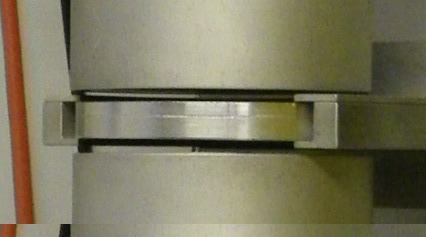
\includegraphics[width=0.5\textwidth]{../pictures/quelle_nah.jpg}
	\caption{Nahaufnahme der genutzten Aluminiumquelle }
	\label{fig:quelle_nah}
\end{figure}


Wenn die Verarbeitung der Aluminiumscheiben bis zum dichten verschließen der Quelle nicht
in Vakuum oder einer Schutzgasathmosphäre stattgefunden hat ist ein oxidieren der äußeren Aluminiumschicht zu erwarten. Die durch das $^{22}$Na
emittierten Positronen treffen also zunächst auf Aluminiumoxid bevor im inneren Teil der Probe wieder reines Aluminium vorherrscht. In Aluminiumoxid
ist die Bildung von Positronium möglich \cite{PhysRevB.70.115410} hierbei spielen insbesonder Randeffekte an der Oberfläche und in Poren im
Aluminiumoxid eine wichtige Rolle die energetischen Bedingungen für die Erzeugung von Positronium zu erzeugen \cite{phd_trezzi}. Man geht von
einer Rückdiffusion der Positronen aus dem Material aus bei dem ein anschließender Einfang eines Elektrons aus der Randschicht 
(hier kann die Probenoberfläche oder der Rand einer Pore gemeint sein) erfolgt.

Die Analyse für Aluminium wird mit den gleichen Methoden wie für Polyethylen durchgeführt, wenn auch für die
Beschreibung der Methoden auf Kapitel \ref{cap:poly} verwiesen wird.
\subsection{Zwei lineare Anpassungen}
\begin{table}[h]
	\begin{tabular}{l |l l ||l}
			Fit& Bereich $[\si{ns}]$ & $τ [\si{ns}]$ & $τ_\text{ges} [\si{ns}]$ \\
		\hline
		\multirow{3}{*}{1} & 0.6 - 1.7 &  0.6193 ± 0.0027   &\multirow{3}{*}{  0.6234 ± 0.0096}\\
	 & 0.6 - 1.5 &  0.6142 ± 0.0032   &\\
	 & 0.8 - 2.0 &  0.6367 ± 0.003   &\\
	 \hline
	 \multirow{3}{*}{2}  & 2.9 - 7.0 &  1.969 ± 0.019   &\multirow{3}{*}{1.965 ± 0.074 }\\
	 & 2.9 - 6 &  1.872 ± 0.023   &\\
	 & 3.5 - 7.0 &  2.054 ± 0.029   &
	\end{tabular}
	\centering
	\caption{Ergebnisse für die Lebensdauer von Positronen in Aluminium mit zwei linearen
		Geradenanpassungen. Da die Werte nicht miteinander vereinbar sind, wird der Mittelwert und
	RMS für die Werte bestimmt.}
	\label{tab:linearPoly}
\end{table}
\subsection{Globale Anpassung an Faltungsfunktion}

\begin{table}[h]
	\begin{tabular}{l |l l}
		Bereich [$\si{ns}$] & $τ_1 [\si{ns}]$ & $τ_2 [\si{ns}]$ \\
		\hline
0.2 - 7 &  0.4771 ± 0.0063   &  2.133 ± 0.029  \\
0.2 - 9 &  0.4979 ± 0.005   &  2.303 ± 0.027  \\
0.9 - 8 &  0.4958 ± 0.006   &  2.296 ± 0.028  \\
		\hline
		\hline
		Mittelung & 0.4903 ± 0.0093 & 2.244 ± 0.079
	\end{tabular}
	\centering
	\caption{Ergebnisse für die Lebensdauer von Positronen in Aluminium mit einer globalen
	Anpassungsfunktion mit variablen Bereichen. Da die Werte nicht oder nur knapp miteinander
		vereinbar sind, wird nicht der gewichtete Mittelwert, sondern Mittelwert und RMS bestimmt.}
	\label{tab:globalPoly}
\end{table}

\FloatBarrier
\subsection{Centroid Shift}
Für Aluminium ergibt sich bei gleicher Vorgehensweise wie bei Polyethylen $τ_1 = 0.5066 \pm 0.0089
\si{ns}$.

\section{Diskussion}
Alle angewandten Messmethoden liefern ähnliche Ergebnisse, eine grafische Zusammenfassung ist in den
Abbildungen \ref{fig:finalt1} und \ref{fig:finalt2} dargestellt.

\begin{figure}[h]
	\includegraphics[width=.5\textwidth]{../analyse/final_plot_1.pdf}
	\includegraphics[width=.5\textwidth]{../analyse/final_plot_2.pdf}
	\caption{Zusammenfassung der Ergebnisse für $\tau_{2}$ }
	\label{fig:finalt2}
\end{figure}

Die bestimmten Fehler scheinen jedoch nicht alle systematische Unsicherheiten ausreichend abzubilden.
Dies führt dazu, dass die präsentierten Ergebnisse teilweise statistisch nicht innerhalb eines $3\sigma$ Intervall
zu einander kompatibel sind (siehe Tabelle \ref{tab:finalsigma}). Insbesondere bei der Bestimmung von $\tau_{1}$ scheint die Bestimmung über eine
lineare Anpassung ein systematische Verschiebung zu größeren Zeiten zu besitzen, weil die Ergebnisse
sowohl für Polyethylen als auch für Aluminium mehr als
$10σ$ von den beiden anderen Messmethoden nach oben verschoben sind, diese aber jeweils innerhalb von
$3σ$ miteinander kompatibel sind.

Bei der Bestimmung von $\tau_{2}$
hingegen liefert die lineare Anpassung ein mit der globalen Anpassung kompatibles Ergebnis. Als Grund für die systematische Abweichung bei der
Bestimmung von $\tau_{1}$ wird der Einfluss der Faltung mit der Auflösungsfunktion angenommen, das Signalspektrum lässt sich hier also im Gegensatz zu längeren
Zeiten nicht ausreichend durch das aufgenommene Spektrum approximieren. Der Einfluss der langlebigen Komponente $\tau_{2}$ auf die lineare Anpassung für $\tau_{1}$
wird auf Grund des, in der globalen Anpassung gewonnenen, Amplitudenverhältnis als vernachlässigbar angesehen.

\begin{table}[h]
	\centering
	\begin{tabular}{c |c |c }
	$\tau_{1}$ & Polyethylen & Aluminium \\
	\hline
	Linearer Fit / Globaler Fit   & 10.85σ & 9.96σ \\
	Linearer Fit / Centroid Shift & 13.96σ & 8.92σ  \\
	Globaler Fit / Centroid Shift &  2.11σ & 1.27σ \\
	\end{tabular}

	\vspace*{0.5cm}
	\begin{tabular}{c |c |c }
	$\tau_{2}$ & Polyethylen & Aluminium\\
	\hline
	Linearer Fit / Globaler Fit\hspace*{0.37cm} & 1.78σ & 2.58σ\\
	\end{tabular}
	\caption{Die Tabelle zeigt wie viele Standardabweichungen die einzelnen Messmethoden für $\tau_{1,2}$ von einander abweichen}
	\label{tab:finalsigma}
\end{table} 
% überall den fehler durch die nullpunktsverschibung von 0.15ns hinzu
\bibliographystyle{plain}
\bibliography{citebib}{}
\end{document}
